\documentclass[border=10pt]{standalone}
\usepackage[svgnames]{xcolor}
\usepackage{amsmath}
\usepackage{pgfplots}
\pgfplotsset{compat=newest}
\usepackage[sfdefault]{FiraSans}
\usepackage{FiraMono}
\renewcommand*\familydefault{\sfdefault}
\begin{document}
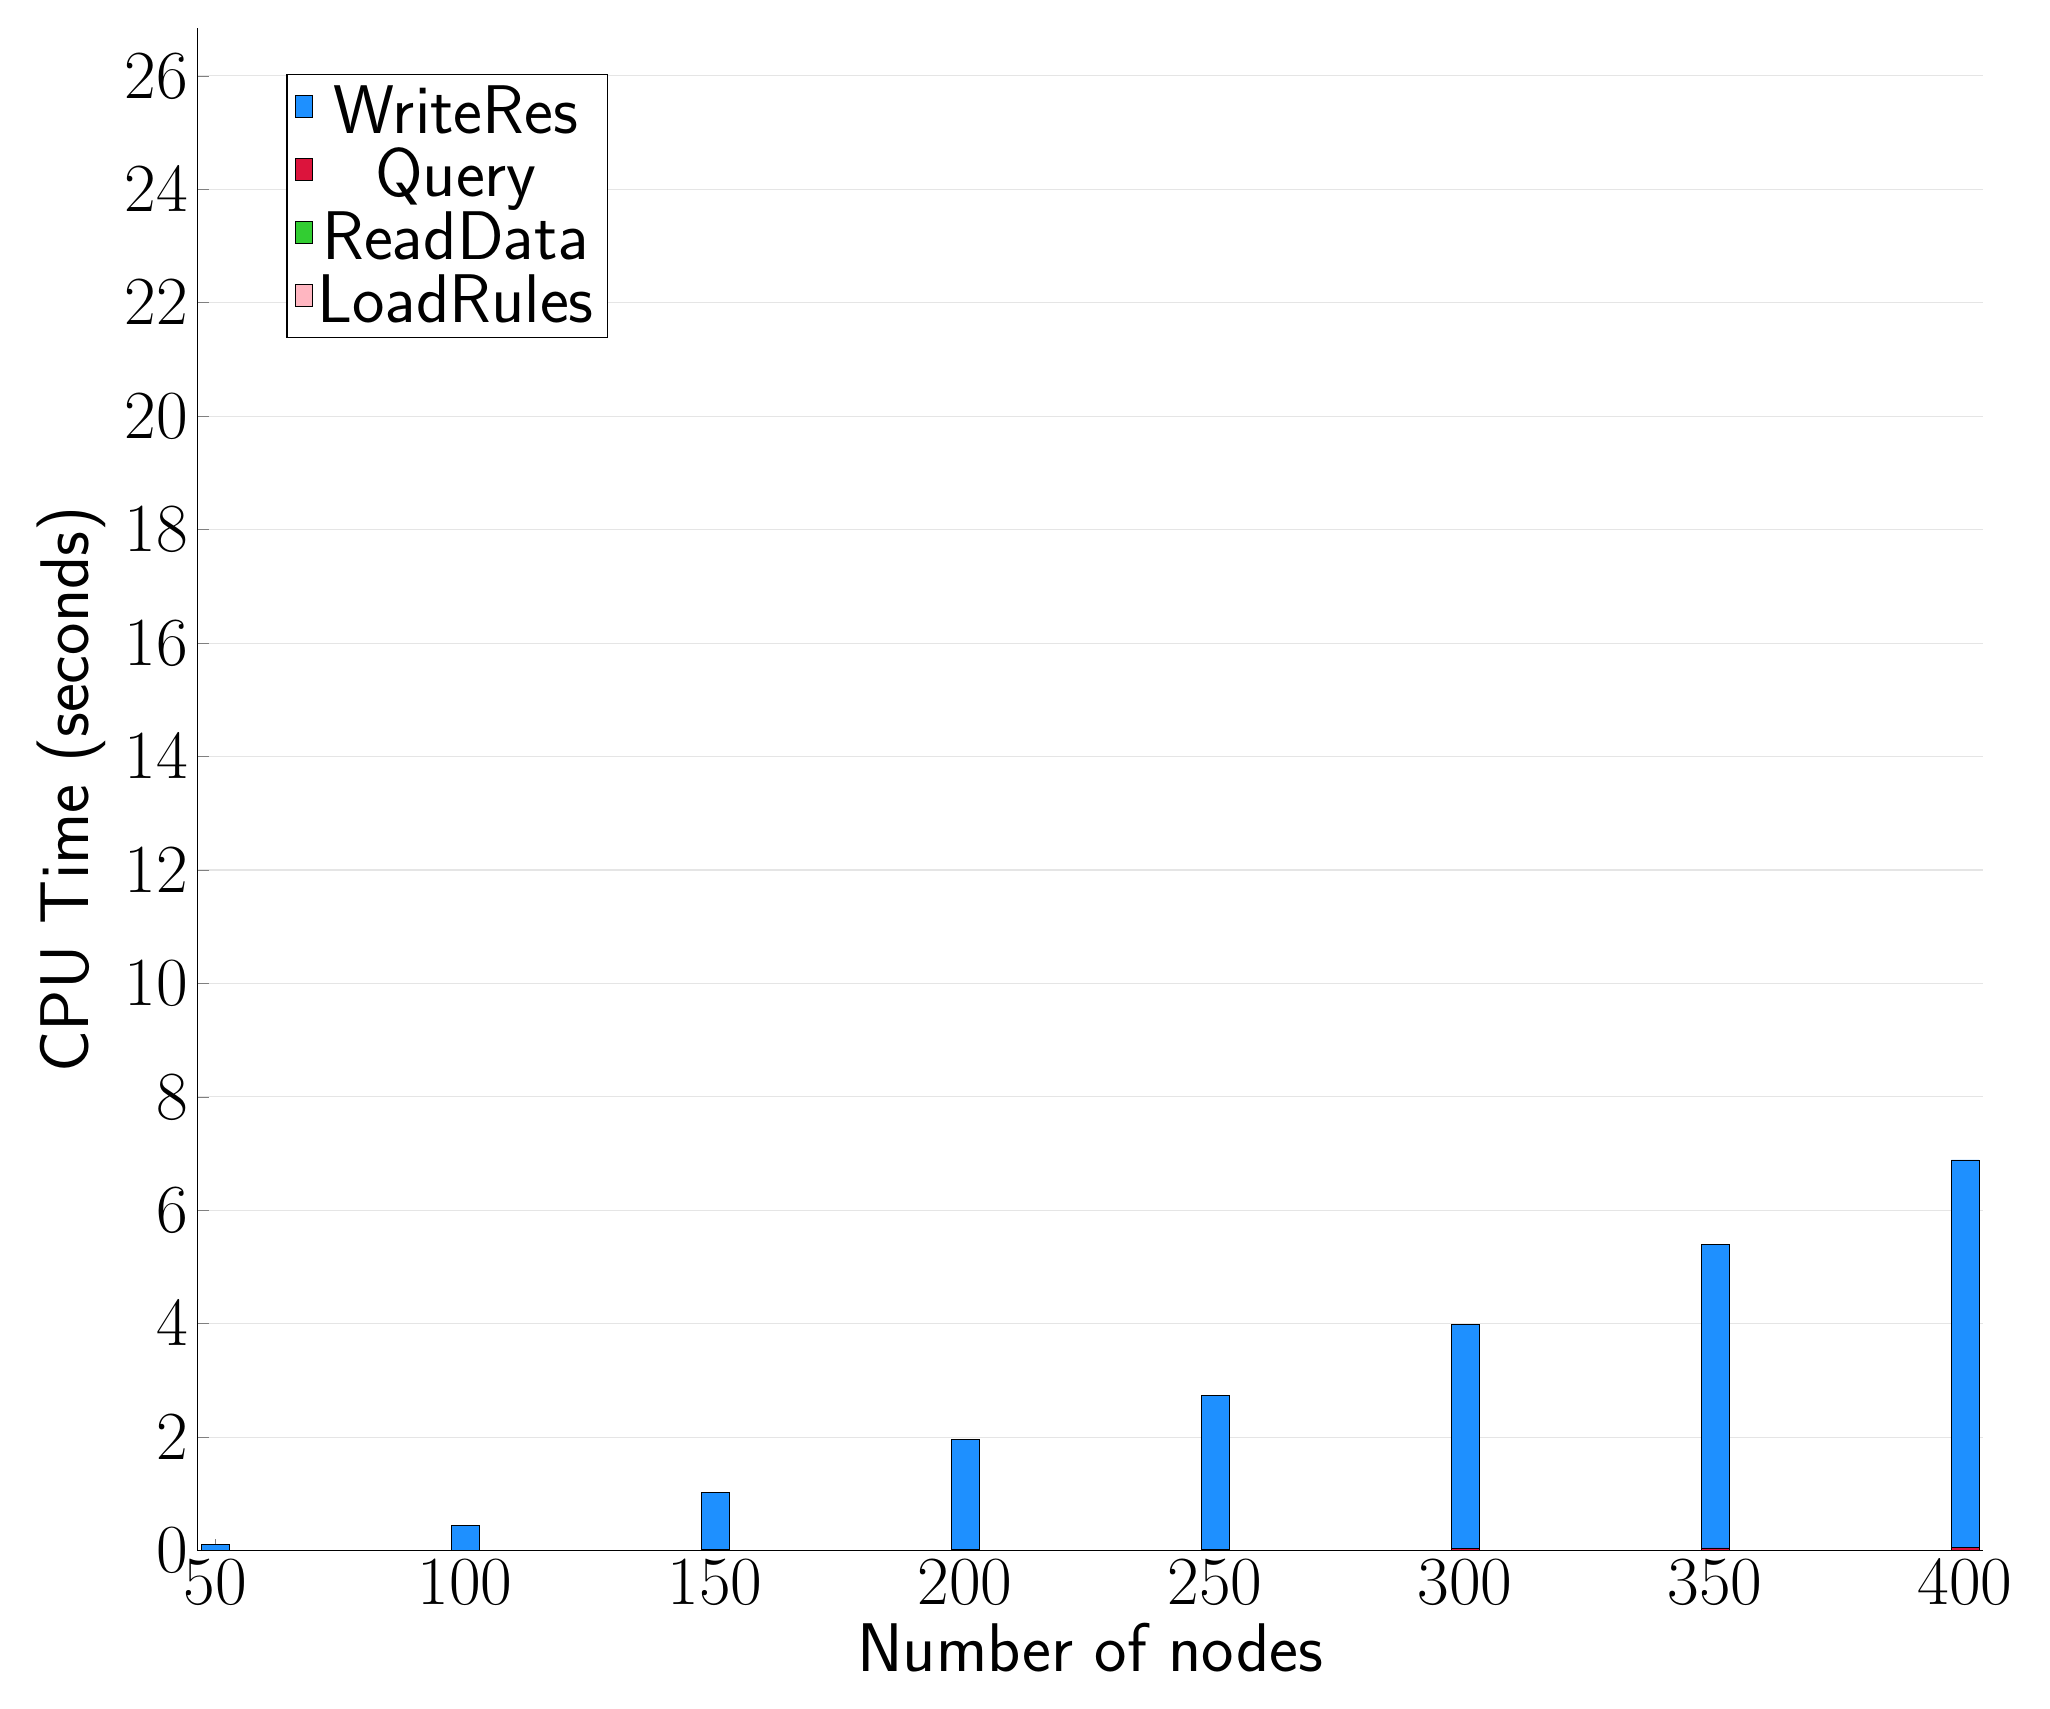
\begin{tikzpicture}
\begin{axis}[
   ybar stacked,
   width=2\textwidth,
   bar width=0.35cm,
   ymajorgrids, tick align=inside,
   major grid style={draw=gray!20},
   xtick=data,
   ymin=0, ymax=26.83928736050924,
   axis x line*=bottom,
   axis y line*=left,
   enlarge x limits=0.01,
   legend style={
       at={(0.23, 0.97)},
       anchor=north east,
       legend columns=1,
       font=\Huge,
   },
   ylabel={CPU Time (seconds)},
   xlabel={Number of nodes},
   label style={font=\Huge},
   tick label style={font=\Huge},
]
\addlegendimage{fill=DodgerBlue, draw=black, line width=0.2pt}
\addlegendentry{WriteRes}
\addlegendimage{fill=Crimson, draw=black, line width=0.2pt}
\addlegendentry{Query}
\addlegendimage{fill=LimeGreen, draw=black, line width=0.2pt}
\addlegendentry{ReadData}
\addlegendimage{fill=LightPink, draw=black, line width=0.2pt}
\addlegendentry{LoadRules}
\addplot +[fill=LightPink, draw=black, line width=0.2pt] coordinates {
(50, 0.0032623333333333324)
(100, 0.004868000000000001)
(150, 0.004373666666666667)
(200, 0.004872666666666667)
(250, 0.0035220000000000004)
(300, 0.004143666666666667)
(350, 0.004025666666666667)
(400, 0.0038170000000000005)
};
\addplot +[fill=LimeGreen, draw=black, line width=0.2pt] coordinates {
(50, 0.0012643333333333332)
(100, 0.0025336666666666632)
(150, 0.0037079999999999965)
(200, 0.004387333333333333)
(250, 0.004609000000000003)
(300, 0.004971333333333337)
(350, 0.005931333333333337)
(400, 0.006979666666666666)
};
\addplot +[fill=Crimson, draw=black, line width=0.2pt] coordinates {
(50, 0.0005426666666666683)
(100, 0.0034166666666666638)
(150, 0.009353)
(200, 0.012476333333333332)
(250, 0.018581333333333335)
(300, 0.029423)
(350, 0.03970066666666667)
(400, 0.053747333333333334)
};
\addplot +[fill=DodgerBlue, draw=black, line width=0.2pt] coordinates {
(50, 0.09972833333333332)
(100, 0.43118233333333333)
(150, 1.008468)
(200, 1.9406740000000002)
(250, 2.7103256666666664)
(300, 3.953121)
(350, 5.356474666666666)
(400, 6.824064333333332)
};
\end{axis}
\end{tikzpicture}

\end{document}
